\subsection{Touch}\label{subsec:touch}
 Die von Terasic zur Verfügung gestellte Datei zur auslesen des Touch ist leider sehr unübersichtlich aufgebaut. Es ist sehr schwierig die darin enthaltenen Funktionen auf das Projekt anzuwenden. Daher entschieden wir uns selbst ein Touch Interrupt Routine zu erstellen. 
 
 Der resistive Touch Display des LT24 LCD Touch Modul ist mit dem AD783 Analoge Devices Chip verbunden. Abbildung \ref{img:AD783_Signalverlauf} zeigt den Signalverlauf des AD783.  Sobald der Touch Display berührt wird löst der Chip am Pen Interrupt Pin ein Interrupt aus, welches vom Nios II detektiert wird. Darauf schreibt der Nios II über die DIN Leitung ins Kontrollregister um eine Messung der X und Y Koordinaten anzufordern. Während des Acquistation Mode werden die X und Y Koordinaten gespeichert und nach der fallenden Flanke des BUSY Signals über die DOUT Leitung dem Nios II übertragen.\cite{AD7843}. 
 
 Für unser Projekt sind wir daran interessiert den Pen Interrupt zu detektieren und die X und Y Koordinaten auszulesen, damit wir sagen können welcher Taster gedrückt worden ist.
 
Das ganze ist im Modul \textit{touch\_isr.c} realisiert. Darin befindet sich eine Funktion \\ \textit{touch\_init(void*context)}. Diese aktiviert das Touch Pen Interrupt  und registriert die Funktion welche durch das Interrupt aufgerufen wird. 
In der Interrupt Service Routine\\ \textit{touch\_isr(void*context)} wird zuerst das Touch Pen Interrupt  deaktiviert. So das in dieser Zeit kein weiteres Interrupt auftreten kann. Nach dem deaktivieren des Interrupts liesst der \textit{alt\_avalon\_spi\_command} die X und Y Koordinaten aus.

\begin{figure}[h!]
	\centering
	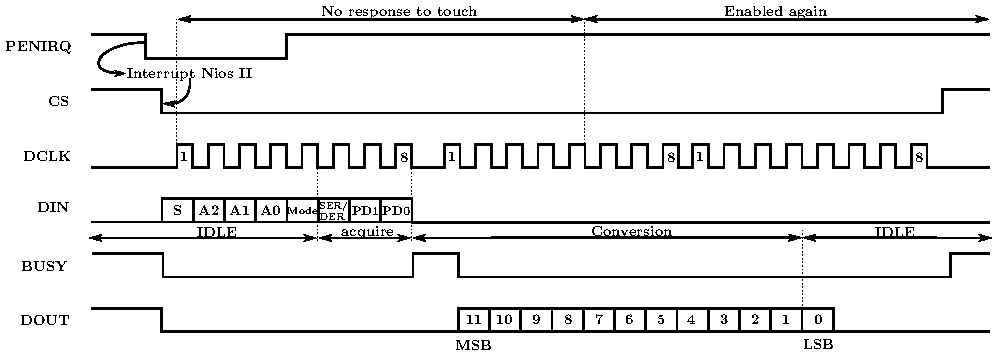
\includegraphics[width=\textwidth]{touch_signal.pdf}
	\caption{Signalverlauf des AD783} 
	\label{img:AD783_Signalverlauf}
\end{figure}  